\documentclass{article}
\usepackage[margin=1in]{geometry}
\usepackage{amsmath,amsthm,amssymb}
\usepackage{bbm,enumerate,mathtools}
\usepackage{tikz,pgfplots}
\usepackage{chessboard}
\usepackage[hidelinks]{hyperref}
\usepackage{multicol} % Problem 35
\usepackage{xstring} % Difficulty command
\usetikzlibrary{shapes.geometric}

\newenvironment{question}{\begin{trivlist}\item[\textbf{Question.}]}{\end{trivlist}}
\newenvironment{note}{\begin{trivlist}\item[\textbf{Note.}]}{\end{trivlist}}
\newenvironment{references}{\begin{trivlist}\item[\textbf{References.}]}{\end{trivlist}}
\newenvironment{related}{\begin{trivlist}\item[\textbf{Related.}]\end{trivlist}\begin{enumerate}}{\end{enumerate}}

\newcommand\score[1]{
\pgfmathsetmacro\pgfxa{#1+1}
\tikzstyle{scorestars}=[
  star,
  star points=5,
  star point ratio=2.25,
  draw,
  inner sep=3pt,
  anchor=outer point 5
]
  \begin{tikzpicture}[baseline]
    \draw[opacity=0] (0,-0.5) rectangle (0,0.2); % Workaround for whitespace at the bottom.
    \foreach \i in {1,...,4} {
      \pgfmathparse{(\i<=#1?"yellow":"gray")}
      \edef\starcolor{\pgfmathresult}
      \draw (\i*4.5ex,0) node[name=star\i,scorestars,fill=\starcolor]  {};
    }
  \end{tikzpicture}
}

\newcommand{\difficulty}[1]{%
  \IfEqCase{#1}{%
      {1}{
        
\begin{tikzpicture}[scale=0.7, baseline=0.9mm]%
          \definecolor{slopegreen}{rgb}{0.0, 0.5, 0.0}%
          \fill[slopegreen] (0.5,0.5) circle (0.5);%
        \end{tikzpicture}%
      }%
      {2}{
        
\begin{tikzpicture}[scale=0.7, baseline=0.9mm]%
          \definecolor{slopeblue}{rgb}{0.0, 0.44, 1.00}
          \fill[slopeblue] (0,0) rectangle (1,1);%
        \end{tikzpicture}%
      }%
      {3}{
\begin{tikzpicture}[scale=0.7, baseline=0.9mm]\fill (0,0.5)--(0.5, 0)--(1,0.5)--(0.5,1)--cycle; \end{tikzpicture}}%
      {4}{
\begin{tikzpicture}[scale=0.7, baseline=0.9mm]\fill (0.25,0)--(0,0.5)--(0.25,1)--(0.5,0.5)--cycle; \fill (0.75,0)--(0.5,0.5)--(0.75,1)--(1,0.5)--cycle;\end{tikzpicture}}%
      % you can add more cases here as desired
  }[\PackageError{difficulty}{Undefined difficulty level: #1}{}]%
}%
\newcommand{\rating}[2]{\difficulty{#1}\\\score{#2}\\}


\begin{document}
\rating{2}{2}
Ezgi showed me a puzzle where dominoes are placed to form a rectangle such that
there is no line that separates the dominoes into two rectangles.
\begin{figure}[ht!]
  \centering
  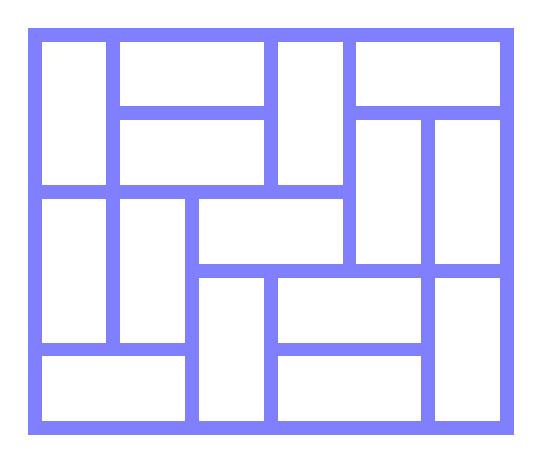
\begin{tikzpicture}
    \draw[blue!50, line width=5]
      (0,6) rectangle (1,4)
      (1,6) rectangle (3,5)
      (3,6) rectangle (4,4)
      (4,6) rectangle (6,5)
      (1,5) rectangle (3,4)
      (4,5) rectangle (5,3)
      (5,5) rectangle (6,3)
      (0,4) rectangle (1,2)
      (1,4) rectangle (2,2)
      (2,4) rectangle (4,3)
      (2,3) rectangle (3,1)
      (3,3) rectangle (5,2)
      (5,3) rectangle (6,1)
      (0,2) rectangle (2,1)
      (3,2) rectangle (5,1);
  \end{tikzpicture}
  \caption{
    The smallest way to place dominoes into a rectangle such that there is no
    way to partition the dominoes into two rectangles.
  }
\end{figure}
\begin{question}
  What size grids have such configurations?
\end{question}

\begin{related}
  \item How many configurations exist for a given grid size?
  \item What if other rectangular polyominoes are used? (e.g. $3 \times 2$ hexominoes)
  \item Are there analogous problems for triangular grids? Higher dimensions?
\end{related}
\end{document}
